\chapter{Specific Requirements}

\section{External Interfaces}~\\
\begin{figure}[H]
    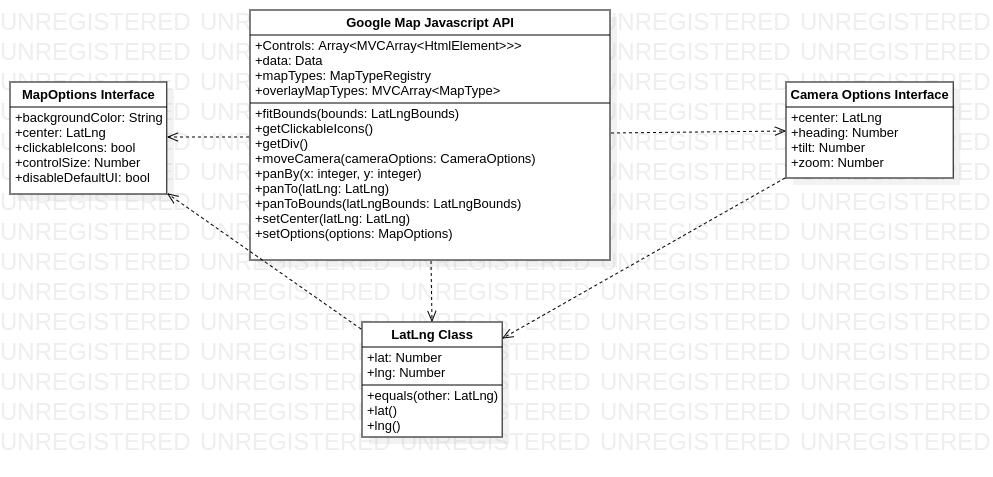
\includegraphics[scale = 0.5]{assets/ExternalInterfaces.png}
    \caption[External Interfaces]{External Interfaces of Afetbilgi.com}
\end{figure}
\section{Functions}
\begin{figure}[H]
    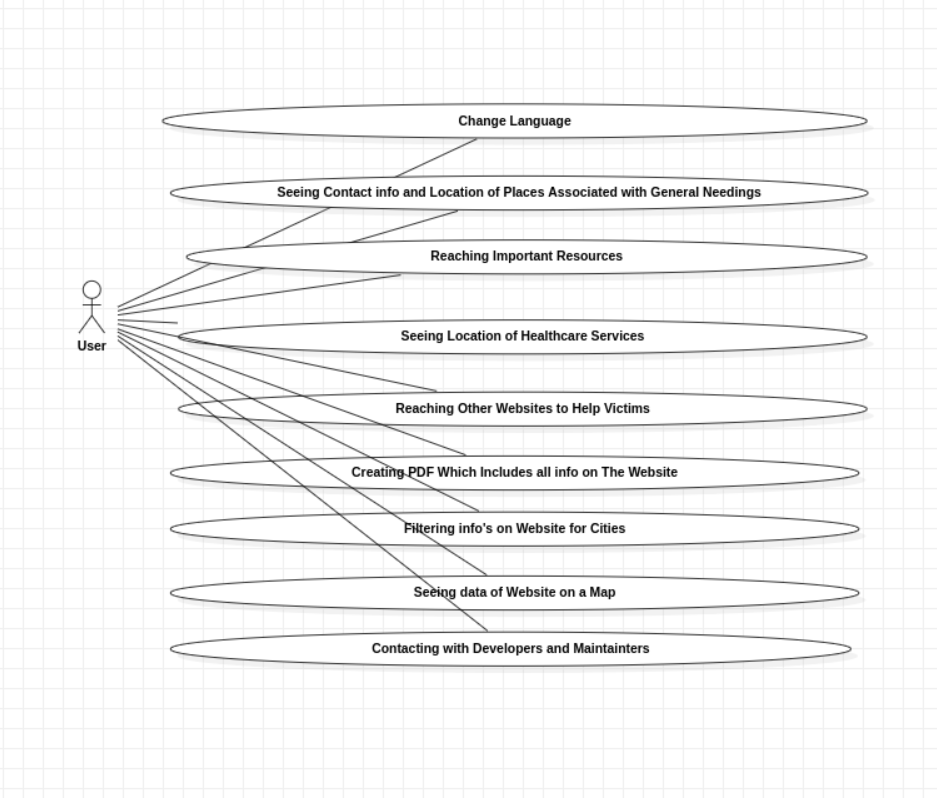
\includegraphics[scale=0.5]{assets/UseCaseDiagram.png}
    \caption[Use Case Diagram]{Use case diagram.}
\end{figure}

\begin{center}
    \begin{table}[H]
        \begin{tabular}{| m{3cm}| m{10cm} |}
            \hline
            \textbf{Use case name}    & Change language                                                                                                           \\
            \hline
            \textbf{Actors}           & User                                                                                                                      \\
            \hline
            \textbf{Description}      & Users can use change button drop menu to change the language of Afetbilgi.com between Turkish, English, Arabic and Kurdi. \\
            \hline
            \textbf{Data}             & -                                                                                                                         \\
            \hline
            \textbf{Preconditions}    & User should be in main page.                                                                                              \\
            \hline
            \textbf{Stimulus}         & User tries to change language.                                                                                            \\
            \hline
            \textbf{Basic flow}       & Step 1 - User opens the languages dropdown menu.                                                                          \\
                                      & Step 2 - User select the language.                                                                                        \\
                                      & Step 3 - React changes the language of page. With selected one.                                                           \\
            \hline
            \textbf{Alternative flow} & -                                                                                                                         \\
            \hline
            \textbf{Exception flow}   & If an error is thrown by react.js it's written on browser console.                                                        \\
            \hline
            \textbf{Postconditions}   & -                                                                                                                         \\
            \hline
        \end{tabular}
        \caption[Change language]{Change language}
    \end{table}
    ~\\~\\~\\
    \begin{table}[H]
        \begin{tabular}{| m{3cm}| m{10cm} |}
            \hline
            \textbf{Use case name}    & Seeing Contact info and Location of general needings                                                                                                           \\
            \hline
            \textbf{Actors}           & User                                                                                                                                                           \\
            \hline
            \textbf{Description}      & Users can find location and contact info (website, phone number etc.) for their general needs like safe gathering places, gas stations, and evacuation points. \\
            \hline
            \textbf{Data}             & Selected city                                                                                                                                                  \\
            \hline
            \textbf{Preconditions}    & -                                                                                                                                                              \\
            \hline
            \textbf{Stimulus}         & User tries to get information about their needs.                                                                                                               \\
            \hline
            \textbf{Basic flow}       & Step 1 - User clicks one of the eight buttons on main page                                                                                                     \\
                                      & Step 2 - User selects a city.                                                                                                                                  \\
                                      & Step 3 - Site returns the table of suitable locations table.                                                                                                   \\
                                      & Step 4 - User clicks one of the links to find further info about location.                                                                                     \\
            \hline
            \textbf{Alternative flow} & Step 1 - User clicks map to open map from main page.                                                                                                           \\
                                      & Step 2 - User finds the desired location from map.                                                                                                             \\
                                      & Step 3 - User clicks the location to get further info.                                                                                                         \\
            \hline
            \textbf{Exception flow}   & If an error occurs on map side, google map API throws an error.                                                                                                \\
            \hline
            \textbf{Postconditions}   & -                                                                                                                                                              \\
            \hline
        \end{tabular}
        \caption[Contact info and location]{Seeing contact info and location of places}
    \end{table}

    ~\\~\\~\\

    \begin{figure}[H]
        \begin{center}
            
\includegraphics[scale=0.5]{assets/ActivityDiagram.png}
            \caption[Activity Diagram of Seeing Contact info and Location of general needings]{Activity Diagram of Seeing Contact info and Location of general needings}
        \end{center}
    \end{figure}

    ~\\~\\~\\

    \begin{table}[H]
        \begin{tabular}{| m{3cm}| m{10cm} |}
            \hline
            \textbf{Use case name}    & Reaching important resources.                                                                                  \\
            \hline
            \textbf{Actors}           & User                                                                                                           \\
            \hline
            \textbf{Description}      & User reach important resources (crucial phone numbers, useful links \& useful articles) from the middle panel. \\
            \hline
            \textbf{Data}             & -                                                                                                              \\
            \hline
            \textbf{Preconditions}    & -                                                                                                              \\
            \hline
            \textbf{Stimulus}         & User tries to get general information about disasters.                                                         \\
            \hline
            \textbf{Basic flow}       & Step 1 - User clicks one of the three buttons on main page                                                     \\
                                      & Step 2 - Site returns table of desired information.                                                            \\
                                      & Step 3 - User can call the desired phone or go to desired website.                                             \\
            \hline
            \textbf{Alternative flow} & -                                                                                                              \\
            \hline
            \textbf{Exception flow}   & -                                                                                                              \\
            \hline
            \textbf{Postconditions}   & -                                                                                                              \\
            \hline
        \end{tabular}
        \caption[Reaching important resources]{Reaching important resources}
    \end{table}
    ~\\~\\~\\
    \begin{table}[H]
        \begin{tabular}{| m{3cm}| m{10cm} |}
            \hline
            \textbf{Use case name}    & Seeing location of healthcare services.                                                                                                                              \\
            \hline
            \textbf{Actors}           & User                                                                                                                                                                 \\
            \hline
            \textbf{Description}      & User can find get the location and some other information about health services (hospitals, pharmacies, veterinarians) from website.                                 \\
            \hline
            \textbf{Data}             & Selected city, (if there is).                                                                                                                                        \\
            \hline
            \textbf{Preconditions}    & -                                                                                                                                                                    \\
            \hline
            \textbf{Stimulus}         & User tries to get information about health services based on their needings.                                                                                         \\
            \hline
            \textbf{Basic flow}       & Step 1 - User clicks one of four buttons from the right frame.                                                                                                       \\
                                      & Step 2 - Site returns a general table if there is no city selected from main menu. If there is a selected city site returns location links of services in this city. \\
                                      & Step 3 - If user didn't filter cities from main menu, now he/she can.                                                                                                \\
                                      & Step 4 - User can reach the location by clicking the location button.                                                                                                \\
            \hline
            \textbf{Alternative flow} & - Step 1 - User can get the location link from map, by filtering by category, by searching or by finding it in map by hand.                                          \\
            \hline
            \textbf{Exception flow}   & -                                                                                                                                                                    \\
            \hline
            \textbf{Postconditions}   & -                                                                                                                                                                    \\
            \hline
        \end{tabular}
        \caption[Location of healthcare services]{Location of healthcare services}
    \end{table}
    ~\\~\\~\\
    \begin{figure}[H]
        \begin{center}
            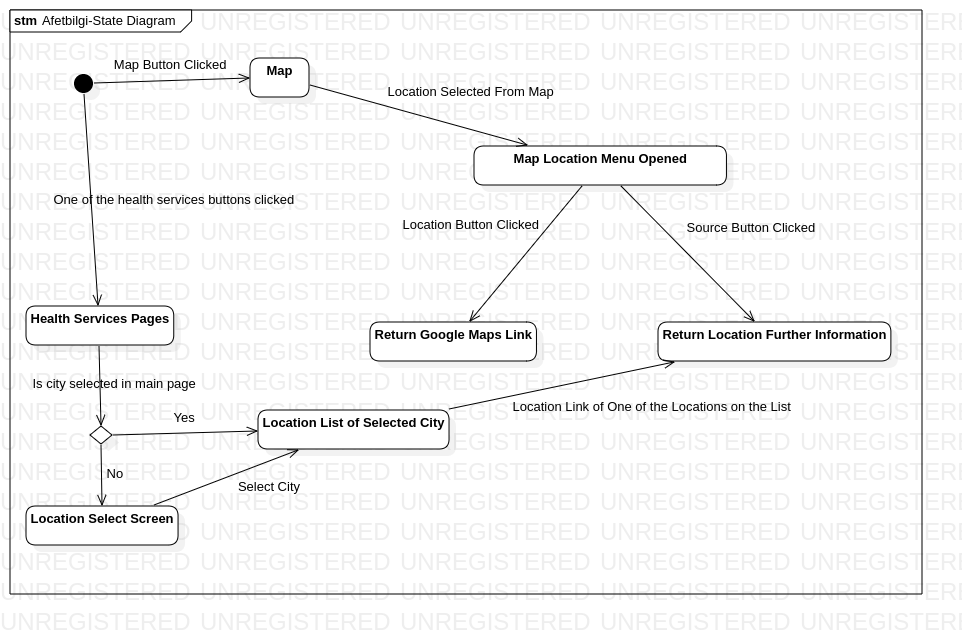
\includegraphics[scale = 0.5]{assets/StateDiagram.png}
            \caption[State Diagram of Getting Locations of Healthcare Services]{State Diagram of Getting Locations of Healthcare Services}
        \end{center}
    \end{figure}

    ~\\~\\~\\
    \begin{table}[H]
        \begin{tabular}{| m{3cm}| m{10cm} |}
            \hline
            \textbf{Use case name}    & Reaching other webistes to help victims.                             \\
            \hline
            \textbf{Actors}           & User                                                                 \\
            \hline
            \textbf{Description}      & User can reach other websites for donating money, blood, stem cell.  \\
            \hline
            \textbf{Data}             & -                                                                    \\
            \hline
            \textbf{Preconditions}    & -                                                                    \\
            \hline
            \textbf{Stimulus}         & User tries to find places or websites to help victims of earthquake. \\
            \hline
            \textbf{Basic flow}       & User clicks one of the 5 buttons on bottom frame of website.         \\
            \hline
            \textbf{Alternative flow} & -                                                                    \\
            \hline
            \textbf{Exception flow}   & -                                                                    \\
            \hline
            \textbf{Postconditions}   & -                                                                    \\
            \hline
        \end{tabular}
        \caption[Reaching other websites]{Reaching other websites}
    \end{table}
    ~\\~\\~\\
    \begin{table}[H]
        \begin{tabular}{| m{3cm}| m{10cm} |}
            \hline
            \textbf{Use case name}    & Creating pdf which includes all info on the website.                                                                                          \\
            \hline
            \textbf{Actors}           & User                                                                                                                                          \\
            \hline
            \textbf{Description}      & User can create a pdf containing the information on website to reach the info offline, or any other purpose.                                  \\
            \hline
            \textbf{Data}             & Selected city. (If there is one).                                                                                                             \\
            \hline
            \textbf{Preconditions}    & -                                                                                                                                             \\
            \hline
            \textbf{Stimulus}         & User tries to get all information of website.                                                                                                 \\
            \hline
            \textbf{Basic flow}       & Step 1 - User clicks download pdf button at the top of the page.                                                                              \\
                                      & Step 2 - Site returns a preformed PDF containing all information about the city (if selected) selected by the user, in the selected language. \\
            \hline
            \textbf{Alternative flow} & -                                                                                                                                             \\
            \hline
            \textbf{Exception flow}   & -                                                                                                                                             \\
            \hline
            \textbf{Postconditions}   & -                                                                                                                                             \\
            \hline
        \end{tabular}
        \caption[Creating pdf]{Creating pdf}
    \end{table}

    ~\\~\\~\\
    \begin{figure}[H]
        \begin{center}
            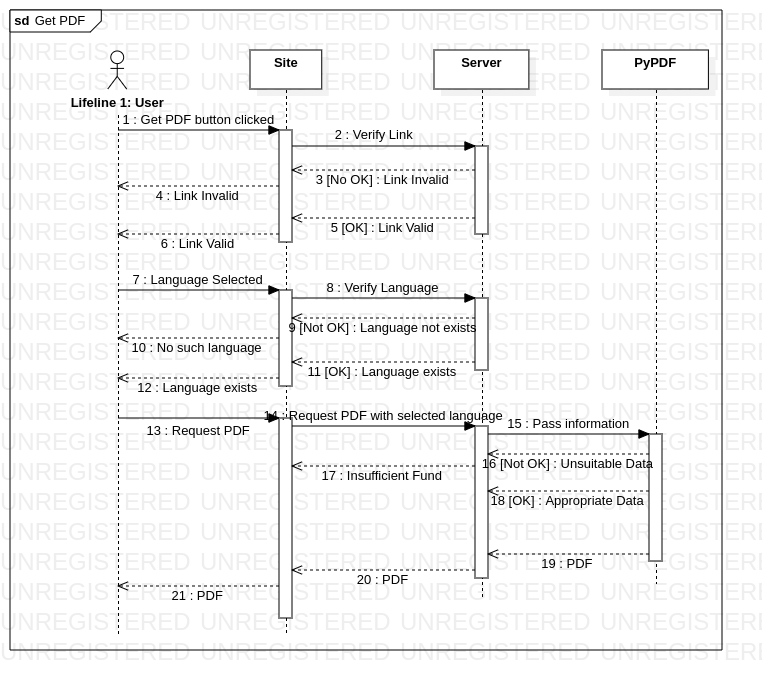
\includegraphics[scale = 0.5]{assets/SequenceDiagram.png}
            \caption[Sequence Diagram of Creating PDF]{Sequence Diagram of Creating PDF}
        \end{center}
    \end{figure}
    ~\\~\\~\\

    \begin{table}[H]
        \begin{tabular}{| m{3cm}| m{10cm} |}
            \hline
            \textbf{Use case name}    & Filtering info's on website for cities.                                                                                                 \\
            \hline
            \textbf{Actors}           & User                                                                                                                                    \\
            \hline
            \textbf{Description}      & User can filter menus and info's on website to include a selected city.                                                                 \\
            \hline
            \textbf{Data}             & Selected city.                                                                                                                          \\
            \hline
            \textbf{Preconditions}    & User should select a city from main menu.                                                                                               \\
            \hline
            \textbf{Stimulus}         & User tries to find relevant information about a city.                                                                                   \\
            \hline
            \textbf{Basic flow}       & Step 1 - User selects a city from main page.                                                                                            \\
                                      & Step 2 - Site filters the main menu. (For example if there is no veterinarian in selected city, user removes the veterinarians button.) \\
                                      & Step 3 - If user goes another page in website, site continues to filter information for the selected city.                              \\
            \hline
            \textbf{Alternative flow} & -                                                                                                                                       \\
            \hline
            \textbf{Exception flow}   & -                                                                                                                                       \\
            \hline
            \textbf{Postconditions}   & -                                                                                                                                       \\
            \hline
        \end{tabular}
        \caption[Filtering information on site by city]{Filtering information on site by city}
    \end{table}
    ~\\~\\~\\
    \begin{table}[H]
        \begin{tabular}{| m{3cm}| m{10cm} |}
            \hline
            \textbf{Use case name}    & Seeing data of website on a map.                                                                                                           \\
            \hline
            \textbf{Actors}           & User                                                                                                                                       \\
            \hline
            \textbf{Description}      & Users can see all locations on website visually in a map and use the map to easily find needed services based on their needs and location. \\
            \hline
            \textbf{Data}             & -                                                                                                                                          \\
            \hline
            \textbf{Preconditions}    & -                                                                                                                                          \\
            \hline
            \textbf{Stimulus}         & User tries to find locations easily.                                                                                                       \\
            \hline
            \textbf{Basic flow}       & Step 1 - User clicks map button at the top of the page.                                                                                    \\
                                      & Step 2 - Site redirects to a map built using Google Map API.                                                                               \\
                                      & Step 3 - User clicks locations or balloons to navigate through map.                                                                        \\
            \hline
            \textbf{Alternative flow} & -                                                                                                                                          \\
            \hline
            \textbf{Exception flow}   & -                                                                                                                                          \\
            \hline
            \textbf{Postconditions}   & -                                                                                                                                          \\
            \hline
        \end{tabular}
        \caption[Seeing data of website on a map]{Seeing data of website on a map}
    \end{table}
    ~\\~\\~\\
    \begin{table}[H]
        \begin{tabular}{| m{3cm}| m{10cm} |}
            \hline
            \textbf{Use case name}    & Contacting with developers and maintainers.                                                               \\
            \hline
            \textbf{Actors}           & User                                                                                                      \\
            \hline
            \textbf{Description}      & Users can find contact info and links to source code and social media accounts of developers from a page. \\
            \hline
            \textbf{Data}             & -                                                                                                         \\
            \hline
            \textbf{Preconditions}    & -                                                                                                         \\
            \hline
            \textbf{Stimulus}         & User wants to reach developers.                                                                           \\
            \hline
            \textbf{Basic flow}       & Step 1 - User clicks About Us / Contact button at the buttom of the page.                                 \\
                                      & Step 2 - Site redirect to a about us page with an Instagram, a twitter and a GitHub link.                 \\
                                      & Step 3 - User can click on of these three buttons or click the mail address to send a mail to developers. \\
            \hline
            \textbf{Alternative flow} & -                                                                                                         \\
            \hline
            \textbf{Exception flow}   & -                                                                                                         \\
            \hline
            \textbf{Postconditions}   & -                                                                                                         \\
            \hline
        \end{tabular}
        \caption[Contacting with developers]{Contacting with developers}
    \end{table}
\end{center}

\section{Usability Requirements}
\begin{itemize}
    \item Site must be usable on both mobile, and desktop browsers.
    \item Users, especially victims should be able to use the site without any background information.
    \item A new data should be added by admins, to the site with at most 3 steps.
    \item Users should be able to use map withoud any location info.
    \item Users should be able to recognize the icons on the map easily.
    \item Victims should be able to get locations and phone numbers without copy paste. Suitable browser APIs should be used.
\end{itemize}

\section{Performance Requirements}
\begin{itemize}
    \item Site must be lightweight, users with bad internet connection should be able to use the site in at most 10 seconds.
    \item Required pdf should be downloaded in 3 seconds.
    \item PDFs should be updated simultaneously when a data is added, removed, or changed.
    \item Map should be lightweight to enable users with old phones to use it without any problem.
\end{itemize}

\section{Logical Database Requirements}
\begin{itemize}
    \item Database should be designed in a way that enables admins to add and remove data's from site.
    \item Database should contain city, county and street information of locations.
    \item Database should contain geographical (WGS84) coordinates of locations to be able to show in map.
\end{itemize}

\section{Design Constraints}
\begin{itemize}
    \item The site must not store any informations about users.
    \item Personal informations such as phone number and address' should be deleted completely after location becomes unavialable.
\end{itemize}

\section{System Attributes}
\subsection{Reliablity}
\begin{itemize}
    \item Failure time of system should be less than 10 minutes in a day.
    \item Site and pdfs should be updated after at most 3 minutes of a database change.
\end{itemize}

\subsection{Availability}
\begin{itemize}
    \item During a restart, the site should be available in 3 minutes.
    \item Data backups should be done in 3 times in a day to prevent a database error.
    \item Site should be available on any device with a browser.
\end{itemize}

\subsection{Security}
\begin{itemize}
    \item Only admins and maintainers should be able to change database.,
    \item Only admins should be able to add a new kind of data to database.
\end{itemize}


\section{Supporting Information}
Even though Afetbilgi is firstly designed for 6 February earthquakes in Turkey, the source code of site is now available in GitHub for further disasters. Developers can download and use the source code of site without any permission.
